%  The AAU Poster Theme.
%  2013-05-08 v. 1.1.0
%  Copyright 2013 by Jesper Kjær Nielsen <jkn@es.aau.dk>
%
%  This is free software: you can redistribute it and/or modify
%  it under the terms of the GNU General Public License as published by
%  the Free Software Foundation, either version 3 of the License, or
%  (at your option) any later version.
%
%  This is distributed in the hope that it will be useful,
%  but WITHOUT ANY WARRANTY; without even the implied warranty of
%  MERCHANTABILITY or FITNESS FOR A PARTICULAR PURPOSE.  See the
%  GNU General Public License for more details.
%
%  You can find the GNU General Public License at <http://www.gnu.org/licenses/>.
\documentclass[a0paper,portrait]{baposter}
\usepackage{xspace}
\usepackage[utf8]{inputenc}
\usepackage[english]{babel}
%\usepackage{helvet}
\renewcommand{\familydefault}{\sfdefault}
\usepackage[T1]{fontenc}
\usepackage{lipsum}
\usepackage{tabularx}
\usepackage[misc]{ifsym}
\usepackage{fixltx2e}
\usepackage{gensymb}

\usepackage{caption}
\captionsetup{
  font=small,% set font size to footnotesize
  labelfont=bf % bold label (e.g., Figure 3.2) font
}

% Make the standard latex tables look so much better
\usepackage{array,booktabs}

% For creating beautiful plots
\usepackage{tikz}
\usetikzlibrary{positioning}
\usetikzlibrary{shapes,arrows,backgrounds,fit,shapes.geometric,calc}
\usetikzlibrary{pgfplots.groupplots}
\usetikzlibrary{patterns}
\usepackage{pgfplots}
\usepackage{pgfplotstable}

\usepackage{amsmath}
\usepackage{amssymb}

% http://en.wikibooks.org/wiki/LaTeX/Colors
\selectcolormodel{RGB}
% define the three aau colors
\definecolor{posterbg}{RGB}{230,230,255}% background colour for the poster

%%%%%%%%%%%%%%%%%%%%%%%%%%%%%%%%%%%%%%%%%%%%%%%%
% Lists
% http://en.wikibooks.org/wiki/LaTeX/List_Structures
%%%%%%%%%%%%%%%%%%%%%%%%%%%%%%%%%%%%%%%%%%%%%%%%
% Easier configuration of lists
\usepackage{enumitem}
%configure itemize
\setlist{%
  topsep=3pt,% set space before and after list
  noitemsep,% remove space between items
  labelindent=\parindent,% set the label indentation to the paragraph indentation
  leftmargin=*,% remove the left margin
  font=\color{black}\normalfont, %set the colour of all bullets, numbers and descriptions to aaublue1
}
\setdescription{font=\color{blue!50!black}\normalfont\bfseries}

%%%%%%%%%%%%%%%%%%%%%%%%%%%%%%%%%%%%%%%%%%%%%%%%
% Misc
%%%%%%%%%%%%%%%%%%%%%%%%%%%%%%%%%%%%%%%%%%%%%%%%
% change/remove some names
\addto{\captionsenglish}{
  %remove the title of the bibliograhpy
  \renewcommand{\refname}{\vspace{-0.7em}}
  %change Figure to Fig. in figure captions
  \renewcommand{\figurename}{Fig.}
}
% create links
\usepackage{url}
%note that the hyperref package is currently incompatible with the baposter class

%%%%%%%%%%%%%%%%%%%%%%%%%%%%%%%%%%%%%%%%%%%%%%%%
% Macros
%%%%%%%%%%%%%%%%%%%%%%%%%%%%%%%%%%%%%%%%%%%%%%%%
\newcommand{\todo}[1]{{\color{red}#1}}
\newcommand{\hilight}[1]{{\color{blue}\textbf #1}}
\newcommand{\julich}{J\"ulich\xspace}
\newcommand{\centerheader}[1]{\begin{center}\bfseries\Large{#1}\end{center} \vspace{-6pt}}
\newcommand{\imageheader}[1]{\begin{center}\bfseries\large{#1}\end{center} \vspace{-2pt}}

\newcommand{\newemph}[1]{{\color{blue!40!black}\em #1}}

\pgfplotsset{every tick label/.append style={font=\footnotesize}}

%%%%%%%%%%%%%%%%%%%%%%%%%%%%%%%%%%%%%%%%%%%%%%%%
% Document Start 
%%%%%%%%%%%%%%%%%%%%%%%%%%%%%%%%%%%%%%%%%%%%%%%%
\begin{document}
%%%%%%%%%%%%%%%%%%%%%%%%%%%%%%%%%%%%%%%%%%%%%%%%
% Some changes that cannot be made in the preamble
%%%%%%%%%%%%%%%%%%%%%%%%%%%%%%%%%%%%%%%%%%%%%%%%
% set the background of the poster
\background{
  \begin{tikzpicture}[remember picture,overlay]%
    %the poster background color
    \fill[fill=white] (current page.north west) rectangle (current page.south east);

    %the header
    \fill [fill=white] (current page.north west) rectangle ([yshift=-\headerheight] current page.north east);
  \end{tikzpicture}
}
% if you want to reduce the space before and after equations, use and adjust
% the following lines
%\addtolength{\abovedisplayskip}{-2mm}
%\addtolength{\belowdisplayskip}{-2mm}

%%%%%%%%%%%%%%%%%%%%%%%%%%%%%%%%%%%%%%%%%%%%%%%%
% General poster setup
%%%%%%%%%%%%%%%%%%%%%%%%%%%%%%%%%%%%%%%%%%%%%%%%
\begin{poster}{
    %general options for the poster
    grid=false,
    columns=3,
    % these two control space between and padding inside
    % the poster boxes
    colspacing=3mm,
    boxpadding=2mm,
    %
    headerheight=0.1\textheight,
    background=user,
    headerborder=closed,
    borderColor=blue!40!black,
    headershape=rectangle,
    headershade=plain,
    headerColorOne=blue!15,
    textborder=rectangle,
    boxshade=plain,
    boxColorOne=white,
    headerFontColor=black,
    headerfont=\Large\sf,
    linewidth=1pt
}

%the Eye Catcher (the logo on the left)
{
  \begin{tikzpicture}[remember picture, overlay]
    \node [anchor=north west,xshift=0.02\paperwidth,yshift=-0.03\headerheight] at (current page.north west) {
      
\includegraphics[height=0.4\headerheight]{HBP_logo.jpg}
    };
    \node [anchor=north west,xshift=0.34\paperwidth,yshift=-0.10\headerheight] at (current page.north west) {
      
\includegraphics[height=0.25\headerheight]{julich_logo.pdf}
    };
    \node [anchor=north west,xshift=0.5\paperwidth,yshift=-0.10\headerheight] at (current page.north west) {
      
\includegraphics[height=0.25\headerheight]{nest-initiative.png}
    };
    \node [anchor=north west,xshift=0.63\paperwidth,yshift=-0.10\headerheight] at (current page.north west) {
      
\includegraphics[height=0.25\headerheight]{cscs_logo.pdf}
    };
    \node[anchor=north west,xshift=0.85\paperwidth,yshift=-0.14\headerheight] at (current page.north west) {
      
\includegraphics[height=0.15\headerheight]{ETHZ_logo.pdf}
    };
  \end{tikzpicture}
  \vspace{0.3\headerheight}
}
%the poster title
{ \Huge
  \textbf{NestMC} \\[0.1\baselineskip]
\large 
  A morphologically detailed neural network simulator for modern high performance computer architectures \\[0.2\baselineskip]
  \small
    Wouter Klijn\textsuperscript{a}, Ben Cumming\textsuperscript{b}, Alexander Peyser\textsuperscript{a}, Vasileios Karakasis\textsuperscript{b}, Stuart Yates\textsuperscript{b} \\
    \textsuperscript{a}Simulation Lab Neuroscience, Forschungszentrum \julich \hspace{2mm}\textsuperscript{b}Swiss National Supercomputing Center  % Would could omit this line, but I guess its best to have it in
}
%the author(s)
{\small
    \vspace{1em} Ben Cumming, \\[0.5em]
    Swiss National Supercomputing Center (CSCS), Switzerland\\
}

%%%%%%%%%%%%%%%%%%%%%%%%%%%%%%%%%%%%%%%%%%%%%%%%
% LEFT HAND SIDE OF POSTER
%%%%%%%%%%%%%%%%%%%%%%%%%%%%%%%%%%%%%%%%%%%%%%%%

%%%%%%%%%%%%%%%%%%%%%%%%%%%%%%%%%%%%%%%%%%%%%%%%
\begin{posterbox}[name=motivation,column=0,row=0,span=2]{Why NestMC?}
    \begin{minipage}[t]{0.3\textwidth}
        \centerheader{Local Field Potential}
        \vspace{4pt}
        \centering
        Both as model output and as part of model feedback loop.
    \end{minipage}
    \hfill
    \begin{minipage}[t]{0.3\textwidth}
        \centerheader{Larger and Longer!}
        \vspace{4pt}
        \centering
        Running more or larger models faster to improve parameter searches and statistical validation.
    \end{minipage}
    \hfill
    \begin{minipage}[t]{0.3\textwidth}
        \vspace{0pt}
        \centerheader{Dynamic Models}
        \vspace{12pt}
        \centering
        Time-varying morphology, connectivity and synapses.
    \end{minipage}

    \imageheader{New and emerging HPC \newemph{many core} architectures can achieve these aims}
   % \vspace{0.5cm}

    \hfill
    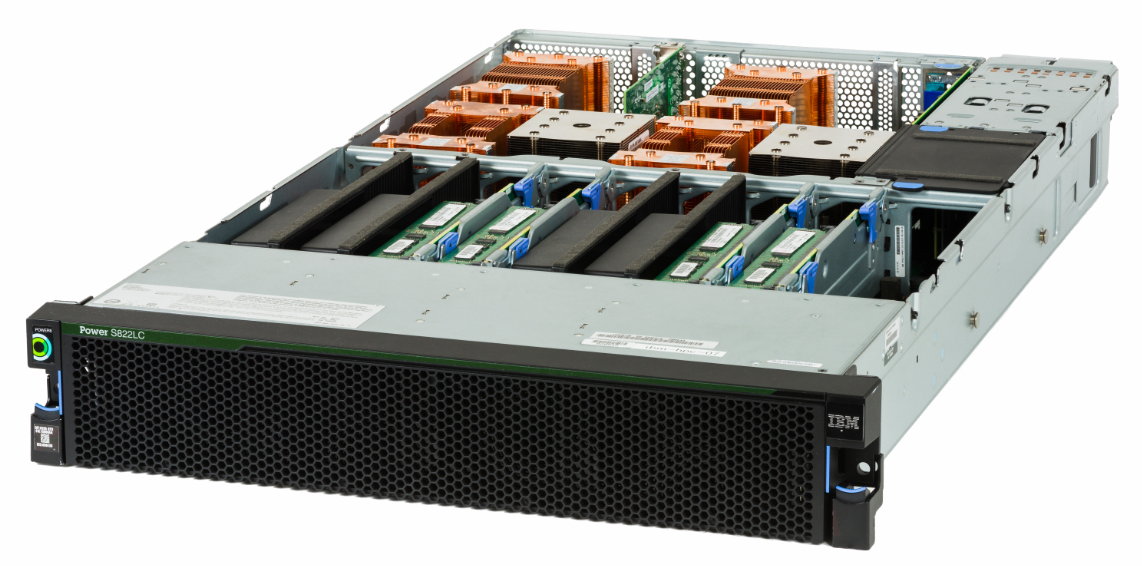
\includegraphics[width=0.35\textwidth]{images/juron.jpg}
    \hfill
    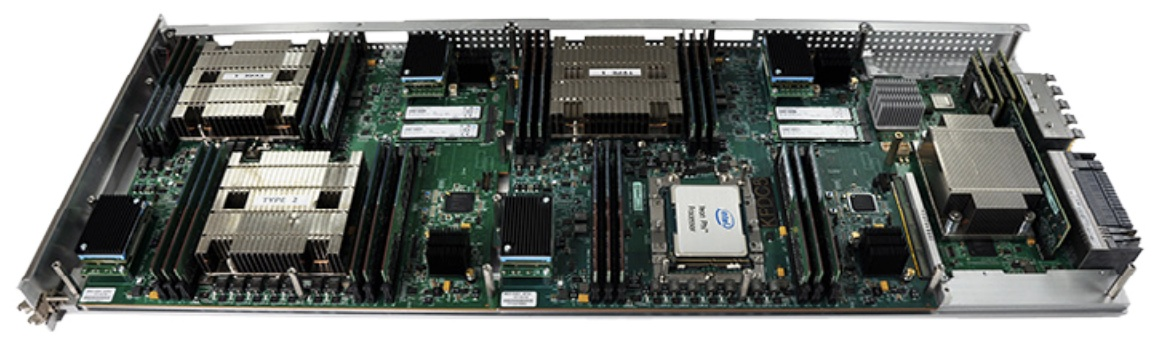
\includegraphics[width=0.55\textwidth]{images/knlnode.jpg}
    \hspace{0.5cm}

    \begin{center}
        Two HBP prototype systems  installed at \julich. Both are a radical departure from current technology.
        \newemph{left}: IBM Power8+GPU ``fat node''. \newemph{right}: Intel many core KNL ``blade''.
    \end{center}

    Current simulators were designed for single core systems, with parallel implementations added later.
    There are efforts to add many core support to existing codes, however they are subject to the law of diminishing returns.
    This presents an opportunity to start work on the next generation of simulators, designed from the ground up to support diverse many core architectures.
    \newemph{NestMC} aims to fill this gap.

\end{posterbox}
%%%%%%%%%%%%%%%%%%%%%%%%%%%%%%%%%%%%%%%%%%%%%%%%

%%%%%%%%%%%%%%%%%%%%%%%%%%%%%%%%%%%%%%%%%%%%%%%%
\begin{posterbox}[name=who,column=0,below=motivation,span=1]{Who}
    \begin{center}
        NestMC is developed by a team from three HPC centers at \julich, CSCS and BSC.
    \end{center}
    \vspace{-10pt}
    \begin{itemize}
        \item Part of HPC infrastructure work package in the \newemph{Human Brain Project}.
        \item With the \newemph{NEST Initiative}.
        \item The centers are motivated to prepare neuroscience users for new HPC architectures.
        \item We provide know-how in computer science, math and software development.
    \end{itemize}
\end{posterbox}

\begin{posterbox}[name=how,column=1,below=motivation,span=1]{How}
    \begin{center}
        NestMC is designed from the ground up\\for \newemph{many core}  architectures.
    \end{center}
    \vspace{-10pt}
    \begin{itemize}
        \item Written in modern C++, CUDA, Intel Threading Building Blocks and HPX.
        \item Is \newemph{open source}.
        \item Uses sound development practices including \newemph{unit testing}, \newemph{continuous Integration}, and \newemph{validation}.
        \item Aims to be user and community-driven: you can help!
    \end{itemize}
\end{posterbox}

\begin{posterbox}[name=nestmc,column=0,below=who,span=2]{Prototype}
    \begin{minipage}[t]{0.42\textwidth}
        \centerheader{Start with a prototype}
         The first step is to develop a \newemph{sufficiently complex} prototype to inform important design considerations:
        \begin{itemize}
            \item Explore the trade-offs between abstraction and performance.
            \item Support for representative architectures:
                  multicore, Intel KNL, and GPU.
            \item The features in the prototype test our assumptions and inform the design:
            \begin{itemize}
                \item Test \newemph{interopability} with an external API (e.g. LFP).
                \item Test the \newemph{extensibility} of the internal API used to implement algorithms (e.g. gap junctions).
                \item Test an exotic \newemph{back end} (e.g. GPU).
            \end{itemize}
            \item Aim to understand the design space and domain before committing to a design.
        \end{itemize}
   \end{minipage}
\hfill
    \begin{minipage}[t]{0.55\textwidth}
        \centerheader{Prototype progress}
            \vspace{-4pt} % because itemize dammit
        \begin{itemize}
            \item Support for x86 and KNL (GPU partially).
            \item Supports NMODL for ion channels and synapses.
            \item Distributed building of networks up to millions of cells.
            \item Finite volume discretization of the cable equation.
            \item Generic network connection model distributed via MPI.
            \item Asynchronous spike communication and computation.
            \item Validated against Neuron.
        \end{itemize}
            \vspace{-8pt} % because itemize dammit
        \centerheader{Internal prototype APIs}
        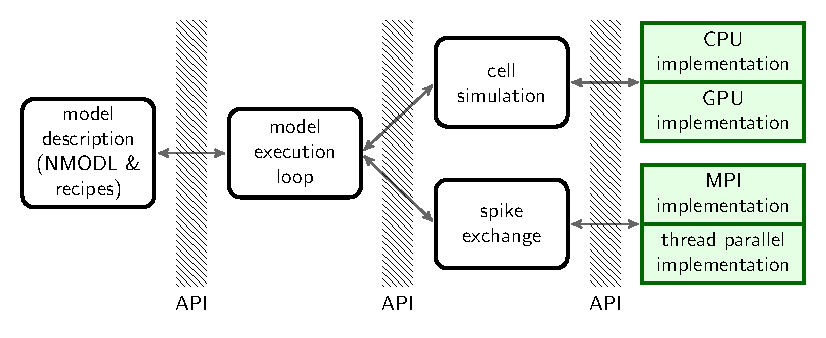
\includegraphics[width=\textwidth]{api.pdf}
            \vspace{-25pt}
        \begin{center}\scriptsize{The modular internal simulation code in the prototype is designed to allow plug and play of different simulation and communication implementations.}\end{center}
   \end{minipage}

\end{posterbox}
%%%%%%%%%%%%%%%%%%%%%%%%%%%%%%%%%%%%%%%%%%%%%%%%

%%%%%%%%%%%%%%%%%%%%%%%%%%%%%%%%%%%%%%%%%%%%%%%%
\begin{posterbox}[name=nestmc,column=0,below=nestmc,span=2]{Do you want to know more?}
\hfill
    \begin{minipage}{0.55\textwidth}
        The source code of the prototype is not in an open repository.
        If you would like to know more, contribute or collaborate, please contact us directly for access to the code.
        \vspace{-13.5pt}
        \begin{center}
            \newemph{The source, tests and validation for NestMC will be in an open repository by April 2017 at the latest.}
        \end{center}
        \vspace{-2.5pt}
    \end{minipage}
\hfill
    \begin{minipage}{0.4\textwidth}
        \colorbox[HTML]{FCF3CF}{%
            \begin{tabularx}{0.9\textwidth}{l|X}
                email & {bcumming@cscs.ch}\\
                      & {a.peyser@fz-juelich.de}\smallskip\\
                web   & {eth-cscs.github.io/nestmc}\smallskip\\
            \end{tabularx}
        }
    \end{minipage}
\hfill

\end{posterbox}
%%%%%%%%%%%%%%%%%%%%%%%%%%%%%%%%%%%%%%%%%%%%%%%%

%%%%%%%%%%%%%%%%%%%%%%%%%%%%%%%%%%%%%%%%%%%%%%%%
% RIGHT HAND SIDE OF POSTER
%%%%%%%%%%%%%%%%%%%%%%%%%%%%%%%%%%%%%%%%%%%%%%%%

%%%%%%%%%%%%%%%%%%%%%%%%%%%%%%%%%%%%%%%%%%%%%%%%
\begin{posterbox}
    [name=help,column=2,row=0,span=1,borderColor=blue!40!black,headerColorOne=blue!40!black,headerFontColor=white]
    {User-driven development is the key!}
        \begin{center}
            \newemph{Current tools and technology influence the ideas that users consider.}

            \vspace{5pt}
        We need help from the neuroscience community.
        \end{center}
            \vspace{-10pt}

        \begin{itemize}\centering
            \item Tell us which features you need.
            \item Help us build a simulator for your community.
        \end{itemize}
\end{posterbox}
%%%%%%%%%%%%%%%%%%%%%%%%%%%%%%%%%%%%%%%%%%%%%%%%

%%%%%%%%%%%%%%%%%%%%%%%%%%%%%%%%%%%%%%%%%%%%%%%%
\begin{posterbox}[name=plots,column=2,below=help,span=1]{Performance of prototype}
        \colorbox[HTML]{FCF3CF}{%
            \begin{tabularx}{0.95\textwidth}{l|X}
                \footnotesize cluster
                    &\footnotesize Cray XC40: 36 cores \& 64\,GB per node\smallskip\\
                \footnotesize cells
                    &\footnotesize 350 compartments \& 2000 synapses each\\
                    &\footnotesize Passive dendrites, Hodgkin–Huxley soma\smallskip\\
                \footnotesize duration
                    &\footnotesize 500\,ms\smallskip\\
            \end{tabularx}
        }
    \vskip4pt
    \imageheader{Reduce wall time with more nodes}
    \tikzset{>=stealth', pil/.style={ ->, color=black!60, thick, } }
\begin{tikzpicture}
    \begin{loglogaxis}[
        height=0.7\textwidth,
        width=\textwidth,
        xmin=1,xmax=512,
        ymin=1, ymax=256,
        xtick={1, 2, 4, 8, 16, 32, 64, 128, 256, 512},
        xticklabels={1, 2, 4, 8, 16, 32, 64, 128, 256, 512},
        %ytick={1,10,100,200},
        ytick={1, 2, 4, 8, 16, 32, 64, 128, 256},
        yticklabels={1,  , 4,  , 16,   , 64, , 256},
        %yticklabels={1,10,100,200},
        ylabel=wall time (s),
        xlabel=nodes,
        xticklabel style={yshift=-2pt},
        yticklabel style={xshift=-2pt},
        legend style = {at={(0,0)}, anchor=south west},
        line width=1.2pt,
        every axis y label/.style=
            {at={(ticklabel cs:0.5)},rotate=90,anchor=near ticklabel},
        grid=major]

        \addplot[color=red, mark=*, mark size=1.5, mark options={fill=white}]
            table[x=nodes,y=gpusmallt] {./images/strong.tbl};
        \addplot[color=blue, mark=triangle*, mark size=1.5, mark options={fill=white}]
            table[x=nodes,y=mcsmallt] {./images/strong.tbl};

        \node[above, fill=red!15, align=center, inner sep=1mm]
           (gsmall) at (axis cs:1.6,40){\tiny 174 s};
        \path[pil,->] (gsmall.north) edge (axis cs:1.05,150);
        \node[above, fill=blue!15, align=center, inner sep=1mm]
           (msmall) at (axis cs:4,128){\tiny 211 s};
        \path[pil,->] (msmall.west) edge (axis cs:1.1,210);

        \node[above, fill=red!15, align=center, inner sep=1mm]
           (gmin) at (axis cs:280,4){\tiny 5.1 s};
        \path[pil,->] (gmin.west) edge (axis cs:140,5);
        \node[above, fill=blue!15, align=center, inner sep=1mm]
           (mmin) at (axis cs:280,1.7){\tiny 2.2 s};
        \path[pil,->] (mmin.west) edge (axis cs:140,2.2);

        \addplot[color=red!40, mark=*, mark size=1.5, mark options={fill=white, solid}]
            table[x=nodes,y=gpubigt] {./images/strong.tbl};
        \addplot[color=blue!40, mark=triangle*, mark size=1.5, mark options={fill=white}]
            table[x=nodes,y=mcbigt] {./images/strong.tbl};

        \node[above, fill=red!15, align=center, inner sep=1mm]
           (glarge) at (axis cs:32,40){\tiny 176 s};
        \path[pil,->] (glarge.north) edge (axis cs:32,155);
        \node[above, fill=blue!15, align=center, inner sep=1mm]
           (mslarge) at (axis cs:128,140){\tiny 204 s};
        \path[pil,->] (mslarge.west) edge (axis cs:35,210);

        \legend{ {\scriptsize gpu 18k},
                 {\scriptsize mc 18k},
                 {\scriptsize gpu 590k},
                 {\scriptsize mc 590k}
               };
    \end{loglogaxis}
\end{tikzpicture}

    { \small
    Time to solution for two models of fixed size as a function of the number of compute nodes.
    Increasing the number of processors reduces the time to solution, with little increase in the compute resources required, measured in \newemph{node hours} (nh).
    }

    \imageheader{Scale out model size}
    \tikzset{>=stealth', pil/.style={ ->, color=black!60, thick, } }
\begin{tikzpicture}
    \begin{semilogxaxis}[
        height=0.7\textwidth,
        width=\textwidth,
        xmin=1,xmax=256,
        ymin=240,ymax=280,
        axis y discontinuity=crunch,
        xtick={1, 2, 4, 8, 16, 32, 64, 128, 256},
        xticklabels={1, 2, 4, 8, 16, 32, 64, 128, 256},
        ytick={250,255,260,265,270,275},
        yticklabels={{~~~250},255,260,265,270,275},
        %yticklabels={50k,100k,150k,200k,250k,300k,350k,400k},
        ylabel=wall time (s),
        xlabel=nodes,
        line width=1.2pt,
        xticklabel style={yshift=-2pt},
        yticklabel style={xshift=-2pt},
        legend style = {at={(0,1)}, anchor=north west},
        every axis y label/.style=
            {at={(ticklabel cs:0.5)},rotate=90,anchor=near ticklabel},
        grid=major]
        \addplot[color=blue, mark=*,mark size=1.5, mark options={fill=white}] table[x=nodes,y=256CPR]
            {./images/scaling_nodes_vs_cpn.tbl};
        \node[above, fill=blue!15, text width=2cm, align=center, inner sep=1mm] (a) at (axis cs:80,272.5){\scriptsize 2,359,296 cells};
        \node[above, fill=blue!15, text width=1.4cm, align=center, inner sep=1mm] (b) at (axis cs:4,270){\scriptsize 9,216 cells};
        \path[pil,->] (a.south) edge (axis cs:230,268.5);
        \path[pil,->] (b.south) edge (axis cs:1.05,263.3);
    \end{semilogxaxis}
\end{tikzpicture}

    { \small
    Time to solution with 256 cells assigned to each core, as the number of nodes is increased.
    This way one can scale up to large networks without significantly increasing wall time (about 9 minutes per simulated second for over 2 million cells on 256 nodes for this model).
    }

    \imageheader{Using high-speed memory on KNL}
    \begin{tikzpicture}
    \begin{semilogyaxis}[
        height=0.7\textwidth,
        width=\textwidth,
        %ymin=0,%ymax=400,
        xmin=1,xmax=16,
        ymin=0.5,ymax=200,
        %xtick={9, 18, 36, 72, 144, 288},
        %xticklabels={9, 18, 36, 72, 144, 288},
        ytick={10,100},
        yticklabels={10,{~~100}},
        ylabel=wall time (s),
        xlabel=fused cells per group,
        line width=1.2pt,
        xticklabel style={yshift=-2pt},
        yticklabel style={xshift=-2pt},
        legend style = {at={(1,0)}, anchor=south east},
        every axis y label/.style=
            {at={(ticklabel cs:0.5)},rotate=90,anchor=near ticklabel},
        grid=major]

        \addplot[color=red, mark=triangle*,mark size=2, mark options={fill=white}] table[x=groupsize,y=largeMCDRAM]
            {./images/knlscaling.tbl};
        \addplot[color=blue,  mark=*,mark size=1.5, mark options={fill=white}] table[x=groupsize,y=smallMCDRAM]
            {./images/knlscaling.tbl};

        \addplot[color=red, dashed, mark=triangle*,mark size=2, mark options={solid, fill=white}] table[x=groupsize,y=largeDDR]
            {./images/knlscaling.tbl};
        \addplot[color=blue, dashed, mark=*,mark size=1.5, mark options={solid, fill=white}] table[x=groupsize,y=smallDDR]
            {./images/knlscaling.tbl};

        %\addplot[color=black,  mark=o,mark size=2] table[x=groupsize,y=largeCACHE]
            %{./images/knlscaling.tbl};
        %\node[left, fill=white] at (axis cs:280,25000){(a)};
        \legend{{\footnotesize 16,384 cells with 1,000 synapses}, {\footnotesize 4,096 cells with 500 synapses}};
    \end{semilogyaxis}
\end{tikzpicture}


    { \small
    Two models are run on KNL with and without high-speed memory (solid and dashed lines respectively).
    The results show the effect of fusing multiple cells into groups, which will be an important optimization for some models and architectures.
    }

\end{posterbox}
%%%%%%%%%%%%%%%%%%%%%%%%%%%%%%%%%%%%%%%%%%%%%%%%

\end{poster}
\end{document}
